%Implementation issues have been briefly discussed in \cite{cui_2016_scalcom}. 
This section presents the details of our rsMPI implementation of Rejuvenating Shadows, as an MPI library. 
Similar to rMPI and RedMPI~\cite{ferreira_sc_2011,fiala_2012_sdc}, rsMPI is implemented as a separate layer between MPI and user application. It uses the standard MPI profiling interface to intercept every MPI call (using function wrappers) and enforces Rejuvenating Shadows logic. 
%In this way, we not only can take advantage of existing MPI performance optimization that numerous researches have spent years on, but also achieve portability across all MPI implementations that conform to the MPI specification.
When used, rsMPI transparently spawns the shadow processes during the initialization phase, manages the coordination between main and shadow processes, and guarantees order and consistency for messages and non-deterministic MPI events.
%Once completed, users should be able to link to the library without any change to existing codes. 

\subsection{MPI rank}
A rsMPI world has 3 types of identities: main process, shadow process, and coordinator process that coordinates between main and shadow. A static mapping between rsMPI rank and application-visible MPI rank is maintained so that each process can retrieve its identity. For example, if the user specifies $N$ processes to run with collocation ratio of 4, rsMPI will translate it into $N + N + N/4$ processes, %where $K$ is the number of shadowed sets. Then the first $N$ ranks will be the mains, the next $N$ ranks be the shadows, and the last $K$ ranks be the coordinators. 
with the first $N$ ranks being the mains, the next $N$ ranks being the shadows, and the last $N/4$ ranks being the coordinators. 
%We also allow the user to specify the collocation of shadows using a configuration file.  Figure~\ref{fig:mapping} shows the mapping between MPI ranks and rsMPI processes for the 3 shadowed sets corresponding to Figure~\ref{fig:logical_org}. 
Using the MPI profiling interface, we added wrapper for MPI\_Comm\_rank() and MPI\_Comm\_size(), so that each process (main or shadow) gets its correct execution path.

%\begin{figure}[!t]
%  \begin{center}
%      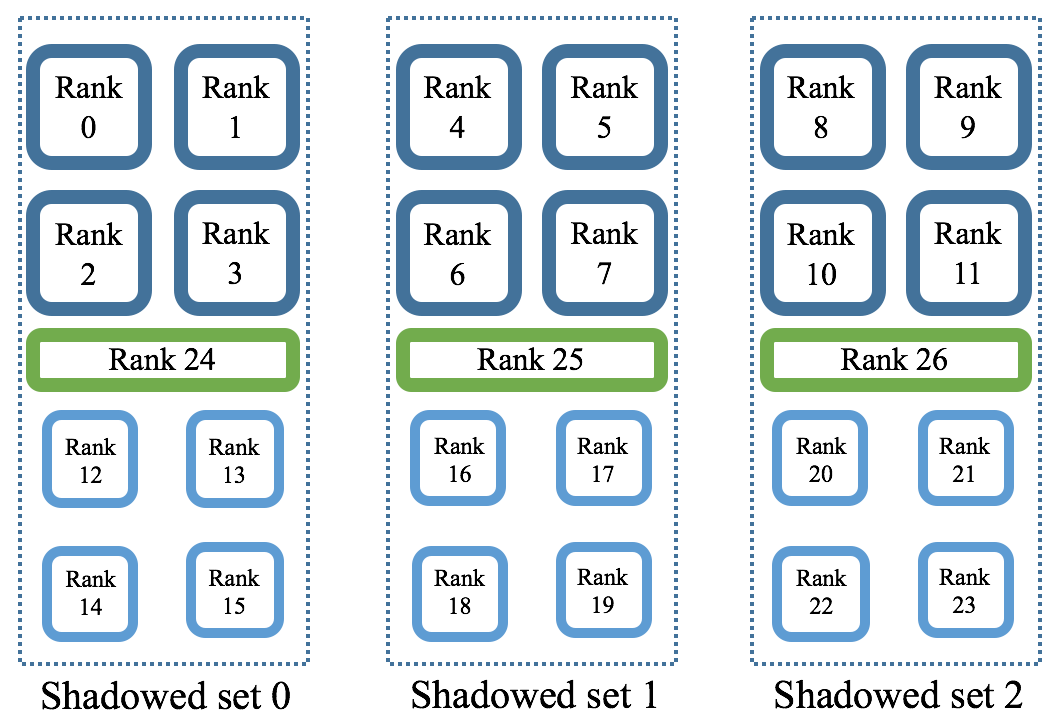
\includegraphics[width=\columnwidth]{figures/mapping}
%  \end{center}
%  \caption{Mapping between MPI ranks and rsMPI processes for an example of 12 application-visible processes grouped into 3 shadowed sets.}
%  \label{fig:mapping}
%\end{figure}

\subsection{Execution rate control}
\label{sec:rate_control}
While each main executes on a separate processor at maximum rate for HPC's throughput consideration, shadows are configured to collocate and execute at a slower rate based on a user configuration file. Accordingly, rsMPI will generate an MPI rankfile and provide it to the MPI runtime to control process mapping. Note that rsMPI always maps the main and shadow of the same task onto different nodes. This is required to prevent a fault on one node from affecting  both a main and its associated  shadow.
%In addition, rsMPI will automatically translate the number of processes (MPI ranks) specified for the application into the number of processes needed by rsMPI. For example, if the user specifies $N$ processes, rsMPI will translate it into $2N + K$ processes, where $K$ is the number of shadowed sets. Therefore, rsMPI will spawn $N$ main processes, $N$ shadow processes, and $K$ shadow coordinator processes for $K$ shadowed sets during MPI initialization. The logical organization is depicted in Figure~\ref{fig:logical_org}. 
To minimize resource usage, each coordinator is collocated with the shadows in the shadowed set. 
A coordinator performs  minimal work, as its main task is to simply handle incoming control messages (discussed below).  As such, the impact of coordinator on the execution rate of collocated shadows is minimal.
%Since a coordinator simply waits for incoming control messages (discussed below) and does minimal work, it has negligible impact on the execution rate of the collocated shadows. 



\subsection{Message passing and consistency}
State consistency between mains and shadows is required both during normal execution and following a failure. % of a main process to roll-forward the shadows. 
As depicted in Figure~\ref{fig:cons_protocol}, a protocol is used 
to enforce sequential consistency, i.e., each shadow sees the same message order and operation results as its main. 
%In this figure, A and B represent two mains, and A' and B' are their shadows. 
Instead of sending messages from main to main and shadow to shadow~\cite{ferreira_sc_2011}, we choose to let the main sender forward each message to the shadow receiver. This allows us to speed up a single shadow when a main fails. 
%For each message, the sending main sends a copy of the message to both the receiving main and its shadow, and the shadow of the sender is suppressed from sending out messages. 
We assume that two copies of the same message are sent in an atomic manner\footnote{This property can be ensured, for example, by using the NIC multicast functionality of the network.}.
%Note that, the SYNC message in Figure~\ref{fig:cons_protocol} is only used to address potential non-determinism as will be discussed in details in the next section.

\begin{figure}[!t]
  \begin{center}
      	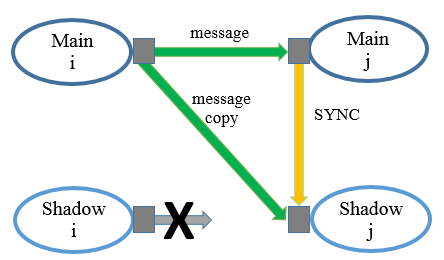
\includegraphics[width=0.7\columnwidth]{figures/cons_protocol_hpcc.png}
  \end{center}
  \vskip -0.2in
  \caption{Consistency protocol for Rejuvenating Shadows.}
  \label{fig:cons_protocol}
  \vskip -0.2in
\end{figure}

For MPI point-to-point communication routines, we add wrappers to implement the above consistency protocol. %For sending functions, such as MPI\_Send() and MPI\_Isend(), rsMPI requires the main to duplicate the sending while the messages are suppressed at the shadow (see Figure~\ref{fig:cons_protocol}). For receiving functions, such as MPI\_Recv() and MPI\_Irecv(), both the main and the shadow does one receiving from the main process at the sending side. 
Collective communication in rsMPI uses point-to-point communication in a binomial tree topology, which demonstrates excellent scalability.
Assuming that only MPI operations can introduce non-determinism, the SYNC message shown in Figure~\ref{fig:cons_protocol} is used to enforce consistency in such cases. For example, MPI\_ANY\_SOURCE may result in different message orders between a main and its shadow. To deal with this, we serialize the receiving of MPI\_ANY\_SOURCE messages by having the main finish the receiving and then use a SYNC message to forward the message source to its shadow, which then receives from the specific source. 
%Other operations, such as MPI\_Wtime() and MPI\_Probe(), are dealt with in a similar manner by forwarding the result from a main to its shadow.

\subsection{Coordination between mains and shadows}
Each shadowed set has a coordinator process dedicated to coordination between the mains and shadows in the set. 
Coordinators do not execute application code, but just wait for rsMPI defined control messages, and then carry out some 
coordination work accordingly. There are three types of control messages: termination, failure, and leaping. They corresponds to three actions:
\begin{itemize}
  \item When a main finishes, the coordinator forces the associated shadow to terminate.
  \item When a main fails, the coordinator temporarily speeds up the associated shadow by suspending the other collocated shadows, until the recovery is done.
  \item When a main initiates a leaping, the coordinator triggers leaping at the associated shadow.
\end{itemize}
%Main and shadow processes can communicate with their coordinator via control messages defined by rsMPI. 
% Firstly, when a main process finishes, it notifies its coordinator, which then forces the associated shadow process to terminate. Secondly, when a main process fails, its associated shadow process needs to catch up, so the coordinator will temporarily suspend the other collocated shadows, and resume their execution once the recovery is done. Lastly, when a main or shadow initiates a leaping, either because of failure or buffer overflow, the coordinator triggers leaping at the associated shadow or main.  
%the RAS system will notify the corresponding shadow coordinator, which then promotes the associated shadow process to a new main process and kills the collocated shadows.
To separate control messages from data messages, rsMPI uses a dedicated MPI communicator for the control messages. This Control Communicator is created by the wrapper to the MPI\_Init call. In addition, to ensure fast response and minimize the number of messages, coordinators also use OS signals to communicate with their collocated shadows. %There are three types of coordination in rsMPI.


\subsection{Leaping}
%Checkpointing/restart requires each process to save its execution state, which can be used later to retrieve the state of the computation. 
%Leaping is similar to saving state in Checkpointing/restart, except that the state is transferred between a pair of main and shadow. 
Different from Checkpointing where the process state is saved, leaping directly transfers process state between a main and its shadow. 
To reduce the size of data involved in saving state, rsMPI borrows the idea from application-level checkpointing~\cite{Beguelin97applicationlevel}, and provides the following API for users to register any data as process state:

\begin{tabular}{ l l}
void & leap\_register\_state(void *addr, int count, \textbackslash \\
& MPI\_Datatype dt);
\end{tabular} \\
For each piece of data to register, three arguments are needed: a pointer to the memory address, the number of data items, and the datatype. 
Application developer could use domain knowledge to identify only necessary state data, or use compiler techniques to automate this~\cite{5160999}. 
%Internally, rsMPI uses a linked list to keep track of all registered data. %After each call of ``leap\_register\_state()", rsMPI will add a node to its internal linked list to record the three parameters. 
%During leaping, the linked list is traversed to retrieve all registered data as the process state.

%Coordination in leaping is simpler than in coordinated checkpointing, since leaping is always between a pair of main and shadow, while all processes need to coordinate for checkpointing. To synchronize the leaping between a main and a shadow, the coordinator in the corresponding shadowed set is involved. For example, when a main detects failure of another main and initiates a leaping, it will send a control message to its coordinator, which then uses a signal to notify the associated shadow to participate in the leaping. 

%Different from Checkpointing where the process state is saved, leaping directly transfers process state between a main and its shadow. 
%Since MPI provides natural support for message passing between processes, 
rsMPI uses MPI messages to transfer process state. Although multiple pieces of data can be registered as a process' state, only a single message needs to be transferred, as MPI supports derived datatypes. To isolate state messages from application messages, rsMPI uses a separate MPI communicator to transfer process state.  
By using a coordinator to synchronize the leaping process and relying on  MPI messages to rapidly transfer process state, the overhead of leaping is minimized. 

%A challenge in leaping lies in the need for maintaining state consistency. 
To make sure a pair of main and shadow stay consistent after a leaping, not only user-defined states should be transferred, but also lower level states, such as program counter and message buffers, need to be correctly updated. Specifically, the leap-recipient needs to satisfy two requirements:  
1) Discard all obsolete messages after the leaping; 2) Resume execution at the same point as the leap-provider. We discuss our solutions below, under the assumption that the application's main body consists of a loop, which is true in most HPC applications. 
%Firstly, after updating its state, the lagging process should resume execution at the same point as the target process. Secondly, the lagging process should discard all obsolete message before resuming normal execution. To address these issues, first we assume that the application's main body consists of a loop, which is true in most cases.

%There is no straightforward way to discard obsolete messages since the message buffer is maintained by MPI runtime and not visible to rsMPI. Hence, 
To correctly discard all obsolete messages, rsMPI borrows the idea of ``determinants" from message logging~\cite{Elnozahy:02:Survey}, and requires every main and shadow to log the metadata (i.e., MPI source, tag, and communicator) for all received messages. Then during leaping, the metadata at the leap-provider is transferred to the leap-recipient, so that the later can combine MPI probe and receive to remove the messages that have been consumed by the former but not by itself.

To resume execution from the same point, we restrict leaping to always occur at certain possible points, and use an internal counter to make sure that both the leap-recipient and leap-provider start leaping from the same point. For example, when a main initiates a leaping, the coordinator will trigger a specific signal handler at the associated shadow. The signal handler does not carry out leaping, but sets a flag for leaping and receives from its main a counter value that indicates the leaping point. %Then, the shadow will check the flag and compare the counter value at every possible leaping point. 
Only when both the flag is set and counter value matches will the shadow start leaping. In this way, it is guaranteed that after leaping the leap-recipient and leap-provider will resume execution from the same point. To balance the trade-off between implementation overhead and flexibility, we choose MPI receive operations as the only possible leaping points. 

 

%Alternatively, we choose to remove obsolete message from message buffer by having the process execute all the skipped MPI communication routines after it finishes leaping. To achieve this, we require the user to define a function for the MPI communication functions used in the application's main body loop. The function should have two parameters to specify the starting and ending index for skipped iterations. In addition, the user needs to register the function with rsMPI with the following library call:

%void leap\_register\_func(void (*func)(int, int));

%To discard all obsolete messages after leaping, the process that updates its process state will call the registered function, for which the two parameters will be automatically specified by rsMPI. Essentially, it executes all the  MPI communication functions from the skipped iterations and consumes all the useless messages.  

%\subsection{Failure injection and detection}
%As one main goal of this work is to achieve fault tolerance, an integrated fault injector is required to evaluate the effectiveness and efficiency of rsMPI to tolerate failures during execution. To produce failures in a manner similar to naturally occurring process failures, our failure injector is designed to be distributed and co-exist with all rsMPI processes. Failure is injected by sending a specific signal to the target process.

%Failure detection is beyond the scope of rsMPI, and we assume the underlying hardware platform has a RAS system that provides this functionality. In our prototype, we emulate a RAS system with a signal handler installed at every main and shadow process. The signal handler catches failure signal from failure injector, and uses a rsMPI defined failure message via a dedicated communicator to notify all other processes of its failure. Similar to ULFM, processes in rsMPI can detect failure only when it does an MPI receive operation. When starting a rsMPI receive, rsMPI checks for failure messages before it does the actual MPI receive operation.

%\subsection{Double in-memory checkpointing}
%We also implemented checkpointing to compare with rsMPI in the presence of failures. To be optimistic, we chose double in-memory checkpointing that is much more scalable then disk-based checkpointing~\cite{zheng2004ftc}. Same as leaping in rsMPI, our implementation provides an API for process state registration. This API requires the same parameters as leap\_register\_state(void *addr, int count, MPI\_Datatype dt), but internally, it needs to allocate extra memory in order to store the state of a ``buddy" process. Another provided API is checkpoint(), which can be used to insert a checkpoint in the application code. For fairness, our implementation also uses MPI messages to transfer state between buddies.  
